\documentclass[doc,floatsintext]{apa6}
\usepackage{lmodern}
\usepackage{amssymb,amsmath}
\usepackage{ifxetex,ifluatex}
\usepackage{fixltx2e} % provides \textsubscript
\ifnum 0\ifxetex 1\fi\ifluatex 1\fi=0 % if pdftex
  \usepackage[T1]{fontenc}
  \usepackage[utf8]{inputenc}
\else % if luatex or xelatex
  \ifxetex
    \usepackage{mathspec}
  \else
    \usepackage{fontspec}
  \fi
  \defaultfontfeatures{Ligatures=TeX,Scale=MatchLowercase}
\fi
% use upquote if available, for straight quotes in verbatim environments
\IfFileExists{upquote.sty}{\usepackage{upquote}}{}
% use microtype if available
\IfFileExists{microtype.sty}{%
\usepackage{microtype}
\UseMicrotypeSet[protrusion]{basicmath} % disable protrusion for tt fonts
}{}
\usepackage{hyperref}
\hypersetup{unicode=true,
            pdftitle={Working with list-columns in data.table},
            pdfauthor={Tyson S. Barrett},
            pdfkeywords={data.table, dplyr, list-columns, nesting},
            pdfborder={0 0 0},
            breaklinks=true}
\urlstyle{same}  % don't use monospace font for urls
\usepackage{color}
\usepackage{fancyvrb}
\newcommand{\VerbBar}{|}
\newcommand{\VERB}{\Verb[commandchars=\\\{\}]}
\DefineVerbatimEnvironment{Highlighting}{Verbatim}{commandchars=\\\{\}}
% Add ',fontsize=\small' for more characters per line
\usepackage{framed}
\definecolor{shadecolor}{RGB}{248,248,248}
\newenvironment{Shaded}{\begin{snugshade}}{\end{snugshade}}
\newcommand{\AlertTok}[1]{\textcolor[rgb]{0.94,0.16,0.16}{#1}}
\newcommand{\AnnotationTok}[1]{\textcolor[rgb]{0.56,0.35,0.01}{\textbf{\textit{#1}}}}
\newcommand{\AttributeTok}[1]{\textcolor[rgb]{0.77,0.63,0.00}{#1}}
\newcommand{\BaseNTok}[1]{\textcolor[rgb]{0.00,0.00,0.81}{#1}}
\newcommand{\BuiltInTok}[1]{#1}
\newcommand{\CharTok}[1]{\textcolor[rgb]{0.31,0.60,0.02}{#1}}
\newcommand{\CommentTok}[1]{\textcolor[rgb]{0.56,0.35,0.01}{\textit{#1}}}
\newcommand{\CommentVarTok}[1]{\textcolor[rgb]{0.56,0.35,0.01}{\textbf{\textit{#1}}}}
\newcommand{\ConstantTok}[1]{\textcolor[rgb]{0.00,0.00,0.00}{#1}}
\newcommand{\ControlFlowTok}[1]{\textcolor[rgb]{0.13,0.29,0.53}{\textbf{#1}}}
\newcommand{\DataTypeTok}[1]{\textcolor[rgb]{0.13,0.29,0.53}{#1}}
\newcommand{\DecValTok}[1]{\textcolor[rgb]{0.00,0.00,0.81}{#1}}
\newcommand{\DocumentationTok}[1]{\textcolor[rgb]{0.56,0.35,0.01}{\textbf{\textit{#1}}}}
\newcommand{\ErrorTok}[1]{\textcolor[rgb]{0.64,0.00,0.00}{\textbf{#1}}}
\newcommand{\ExtensionTok}[1]{#1}
\newcommand{\FloatTok}[1]{\textcolor[rgb]{0.00,0.00,0.81}{#1}}
\newcommand{\FunctionTok}[1]{\textcolor[rgb]{0.00,0.00,0.00}{#1}}
\newcommand{\ImportTok}[1]{#1}
\newcommand{\InformationTok}[1]{\textcolor[rgb]{0.56,0.35,0.01}{\textbf{\textit{#1}}}}
\newcommand{\KeywordTok}[1]{\textcolor[rgb]{0.13,0.29,0.53}{\textbf{#1}}}
\newcommand{\NormalTok}[1]{#1}
\newcommand{\OperatorTok}[1]{\textcolor[rgb]{0.81,0.36,0.00}{\textbf{#1}}}
\newcommand{\OtherTok}[1]{\textcolor[rgb]{0.56,0.35,0.01}{#1}}
\newcommand{\PreprocessorTok}[1]{\textcolor[rgb]{0.56,0.35,0.01}{\textit{#1}}}
\newcommand{\RegionMarkerTok}[1]{#1}
\newcommand{\SpecialCharTok}[1]{\textcolor[rgb]{0.00,0.00,0.00}{#1}}
\newcommand{\SpecialStringTok}[1]{\textcolor[rgb]{0.31,0.60,0.02}{#1}}
\newcommand{\StringTok}[1]{\textcolor[rgb]{0.31,0.60,0.02}{#1}}
\newcommand{\VariableTok}[1]{\textcolor[rgb]{0.00,0.00,0.00}{#1}}
\newcommand{\VerbatimStringTok}[1]{\textcolor[rgb]{0.31,0.60,0.02}{#1}}
\newcommand{\WarningTok}[1]{\textcolor[rgb]{0.56,0.35,0.01}{\textbf{\textit{#1}}}}
\usepackage{graphicx,grffile}
\makeatletter
\def\maxwidth{\ifdim\Gin@nat@width>\linewidth\linewidth\else\Gin@nat@width\fi}
\def\maxheight{\ifdim\Gin@nat@height>\textheight\textheight\else\Gin@nat@height\fi}
\makeatother
% Scale images if necessary, so that they will not overflow the page
% margins by default, and it is still possible to overwrite the defaults
% using explicit options in \includegraphics[width, height, ...]{}
\setkeys{Gin}{width=\maxwidth,height=\maxheight,keepaspectratio}
\IfFileExists{parskip.sty}{%
\usepackage{parskip}
}{% else
\setlength{\parindent}{0pt}
\setlength{\parskip}{6pt plus 2pt minus 1pt}
}
\setlength{\emergencystretch}{3em}  % prevent overfull lines
\providecommand{\tightlist}{%
  \setlength{\itemsep}{0pt}\setlength{\parskip}{0pt}}
\setcounter{secnumdepth}{0}
% Redefines (sub)paragraphs to behave more like sections
\ifx\paragraph\undefined\else
\let\oldparagraph\paragraph
\renewcommand{\paragraph}[1]{\oldparagraph{#1}\mbox{}}
\fi
\ifx\subparagraph\undefined\else
\let\oldsubparagraph\subparagraph
\renewcommand{\subparagraph}[1]{\oldsubparagraph{#1}\mbox{}}
\fi

%%% Use protect on footnotes to avoid problems with footnotes in titles
\let\rmarkdownfootnote\footnote%
\def\footnote{\protect\rmarkdownfootnote}


  \title{Working with list-columns in \texttt{data.table}}
    \author{Tyson S. Barrett\textsuperscript{1}}
    \date{}
  
\shorttitle{List-columns in data.table}
\affiliation{
\vspace{0.5cm}
\textsuperscript{1} Utah State University}
\keywords{data.table, dplyr, list-columns, nesting}
\usepackage{csquotes}
\usepackage{upgreek}
\captionsetup{font=singlespacing,justification=justified}

\usepackage{longtable}
\usepackage{lscape}
\usepackage{multirow}
\usepackage{tabularx}
\usepackage[flushleft]{threeparttable}
\usepackage{threeparttablex}

\newenvironment{lltable}{\begin{landscape}\begin{center}\begin{ThreePartTable}}{\end{ThreePartTable}\end{center}\end{landscape}}

\makeatletter
\newcommand\LastLTentrywidth{1em}
\newlength\longtablewidth
\setlength{\longtablewidth}{1in}
\newcommand{\getlongtablewidth}{\begingroup \ifcsname LT@\roman{LT@tables}\endcsname \global\longtablewidth=0pt \renewcommand{\LT@entry}[2]{\global\advance\longtablewidth by ##2\relax\gdef\LastLTentrywidth{##2}}\@nameuse{LT@\roman{LT@tables}} \fi \endgroup}


\usepackage{lineno}

\linenumbers

\authornote{

Correspondence concerning this article should be addressed to Tyson S. Barrett, 2800 Old Main, Logan, UT 84322. E-mail: \href{mailto:tyson.barrett@usu.edu}{\nolinkurl{tyson.barrett@usu.edu}}}

\abstract{
The use of \emph{list-columns} in data frames and tibbles in the R statistical environment is well documented (e.g.~Bryan, 2018), providing a cognitively efficient way to organize results of complex data (e.g.~several statistical models, groupings of text, data summaries, or even graphics) with corresponding data. For example, one can store student information within classrooms, player information within teams, or even analyses within groups. This allows the text to be of variable sizes without overly complicating or adding redundancies to the structure of the data. In turn, this can reduce the difficulty to appropriately analyze the data stored in the list-column. Because of its efficiency and speed, being able to use \texttt{data.table} to work with list-columns would be beneficial in many data contexts (i.e.~to reduce memory usage in large data sets). I show how one can create list-columns in a data table using the \texttt{by} argument in \texttt{data.table} and \texttt{purrr::map()}. This is done using an example data set on professional basketball player information. I compare the behavior of the \texttt{data.table} approach to the \texttt{dplyr::group\_nest()} function. Results using \texttt{bench::mark()} show the speed and efficiency of using \texttt{data.table} to work with list-columns.


}

\begin{document}
\maketitle

\hypertarget{introduction}{%
\section{Introduction}\label{introduction}}

The use of \emph{list-columns} in data frames and tibbles in the R statistical environment (R Core Team, 2018) provides a cognitively efficient way to organize complex data (e.g.~several statistical models, groupings of text, data summaries, or even graphics) with corresponding data in a concise manner. It has become a common approach to wrangling data in the \texttt{tidyverse}, with functions across \texttt{dplyr} and \texttt{tidyr} providing functionality to work with list-columns (Bryan, 2018; Wickham et al., 2019; Wickham \& Henry, 2019).

This format is often called \enquote{nested} data, where information is, in essence, nested within a column of data. For example, one can store individual words of a verse in a list for each verse, chapter, book, and volume. This allows the text to be of variable sizes without overly complicating or adding redundancies to the structure of the data.

List-columns can also be used to nest students within classrooms, players within teams, and measures within individuals. This allows the user to do certain data manipulations or analyses within each group. This can ensure that accidentally including data from other groups does not occur. Furthermore, nesting can reduce the difficulty to appropriately analyze the data stored in the list-column. Using functions like \texttt{lapply()} or \texttt{purrr::map*()} makes further analysis of the nested data more intuitive and error-free.

Because of its efficiency and speed, being able to use \texttt{data.table} to work with list-columns would be beneficial in many data contexts (i.e.~to reduce memory usage in large data sets). Herein, I show how one can create list-columns in a data table using \texttt{purrr::map()} and the \texttt{by} argument in \texttt{data.table}. I further highlight the \texttt{dplyr::group\_nest()} function and show a slightly more efficient approach when using a data table. Results using \texttt{bench::mark()} show the speed and efficiency of using \texttt{data.table} to work with list-columns.

This article relies on several powerful packages, including \texttt{data.table}, \texttt{dplyr}, \texttt{bench}, \texttt{tidyr}, \texttt{papaja}, \texttt{stringr}, \texttt{ggplot2}, \texttt{ggbeeswarm}, \texttt{performance}, \texttt{rvest}, and \texttt{lobstr} (Aust \& Barth, 2018; Clarke \& Sherrill-Mix, 2017; Dowle \& Srinivasan, 2019; Hester, 2019; Lüdecke, Makowski, \& Waggoner, 2019; Wickham, 2016, 2019c, 2019b, 2019a; Wickham et al., 2019; Wickham \& Henry, 2019).

\hypertarget{example-data}{%
\section{Example Data}\label{example-data}}

Throughout much of this paper, I will demonstrate the use of \emph{list-columns} in \texttt{data.table} using data from \href{nbastuffer.com}{NBA Stuffer} will be scraped to get information on players from the 2017-2018 and 2018-2019 seasons. First, the HTML data are read in, the tables with player data by year are then extracted using a custom function, indicators are added, and then combined into a single data table for the player data.

\begin{Shaded}
\begin{Highlighting}[]
\NormalTok{url_}\DecValTok{2018}\NormalTok{ <-}\StringTok{ "https://www.nbastuffer.com/2017-2018-nba-player-stats/"}
\NormalTok{url_}\DecValTok{2019}\NormalTok{ <-}\StringTok{ "https://www.nbastuffer.com/2018-2019-nba-player-stats/"}
\NormalTok{players_}\DecValTok{2018}\NormalTok{ <-}\StringTok{ }\KeywordTok{read_html}\NormalTok{(url_}\DecValTok{2018}\NormalTok{)}
\NormalTok{players_}\DecValTok{2019}\NormalTok{ <-}\StringTok{ }\KeywordTok{read_html}\NormalTok{(url_}\DecValTok{2019}\NormalTok{)}

\NormalTok{extract_fun <-}\StringTok{ }\ControlFlowTok{function}\NormalTok{(html)\{}
  \KeywordTok{html_nodes}\NormalTok{(html, }\StringTok{"table"}\NormalTok{)[}\DecValTok{2}\NormalTok{] }\OperatorTok\StringTok{ }
\StringTok{    }\KeywordTok{html_table}\NormalTok{(}\DataTypeTok{fill =} \OtherTok{TRUE}\NormalTok{) }\OperatorTok\StringTok{ }
\StringTok{    }\NormalTok{.[[}\DecValTok{1}\NormalTok{]] }
\NormalTok{\}}

\NormalTok{player_}\DecValTok{2018}\NormalTok{ <-}\StringTok{ }
\StringTok{  }\KeywordTok{extract_fun}\NormalTok{(players_}\DecValTok{2018}\NormalTok{) }\OperatorTok\StringTok{ }
\StringTok{  }\KeywordTok{mutate}\NormalTok{(}\DataTypeTok{year =} \DecValTok{2018}\NormalTok{,}
         \DataTypeTok{AGE =} \KeywordTok{as.numeric}\NormalTok{(AGE))}
\NormalTok{player_}\DecValTok{2019}\NormalTok{ <-}\StringTok{ }
\StringTok{  }\KeywordTok{extract_fun}\NormalTok{(players_}\DecValTok{2019}\NormalTok{) }\OperatorTok\StringTok{ }
\StringTok{  }\KeywordTok{mutate}\NormalTok{(}\DataTypeTok{year =} \DecValTok{2019}\NormalTok{)}

\NormalTok{players <-}\StringTok{ }
\StringTok{  }\KeywordTok{bind_rows}\NormalTok{(player_}\DecValTok{2018}\NormalTok{, player_}\DecValTok{2019}\NormalTok{) }\OperatorTok\StringTok{ }
\StringTok{  }\KeywordTok{clean_names}\NormalTok{() }\OperatorTok\StringTok{ }
\StringTok{  }\KeywordTok{rename}\NormalTok{(}\DataTypeTok{ppg =}\NormalTok{ ppg_points_points_per_game,}
         \DataTypeTok{apg =}\NormalTok{ apg_assists_assists_per_game) }\OperatorTok\StringTok{ }
\StringTok{  }\KeywordTok{data.table}\NormalTok{()}
\end{Highlighting}
\end{Shaded}

\noindent Below is a subset of this imported data set, showing only four of the variables and the first six rows.

\begin{verbatim}
##         full_name  mpg  ppg apg
## 1:   Aaron Brooks  5.9  2.3 0.6
## 2:   Aaron Gordon 32.9 17.6 2.3
## 3: Aaron Harrison 25.9  6.7 1.2
## 4:  Aaron Jackson 34.5  8.0 1.0
## 5:    Abdel Nader 10.9  3.0 0.5
## 6:  Adreian Payne  8.5  4.2 0.0
\end{verbatim}

\hypertarget{nesting-with-data.table}{%
\section{\texorpdfstring{Nesting with \texttt{data.table}}{Nesting with data.table}}\label{nesting-with-data.table}}

In \texttt{dplyr} the \texttt{group\_nest()} function is valuable when creating list-columns based on a grouping variable. It takes the data by group and puts it all in a list-column. Figure \ref{process} highlights the process of taking a data frame and creating a nested data frame with a list-column. That is, all data from variables \texttt{x}, \texttt{y}, and \texttt{z} relating to each group is split into a distinct data frame and stored within the \texttt{data} column.

\begin{figure}[tb]
  \centering
  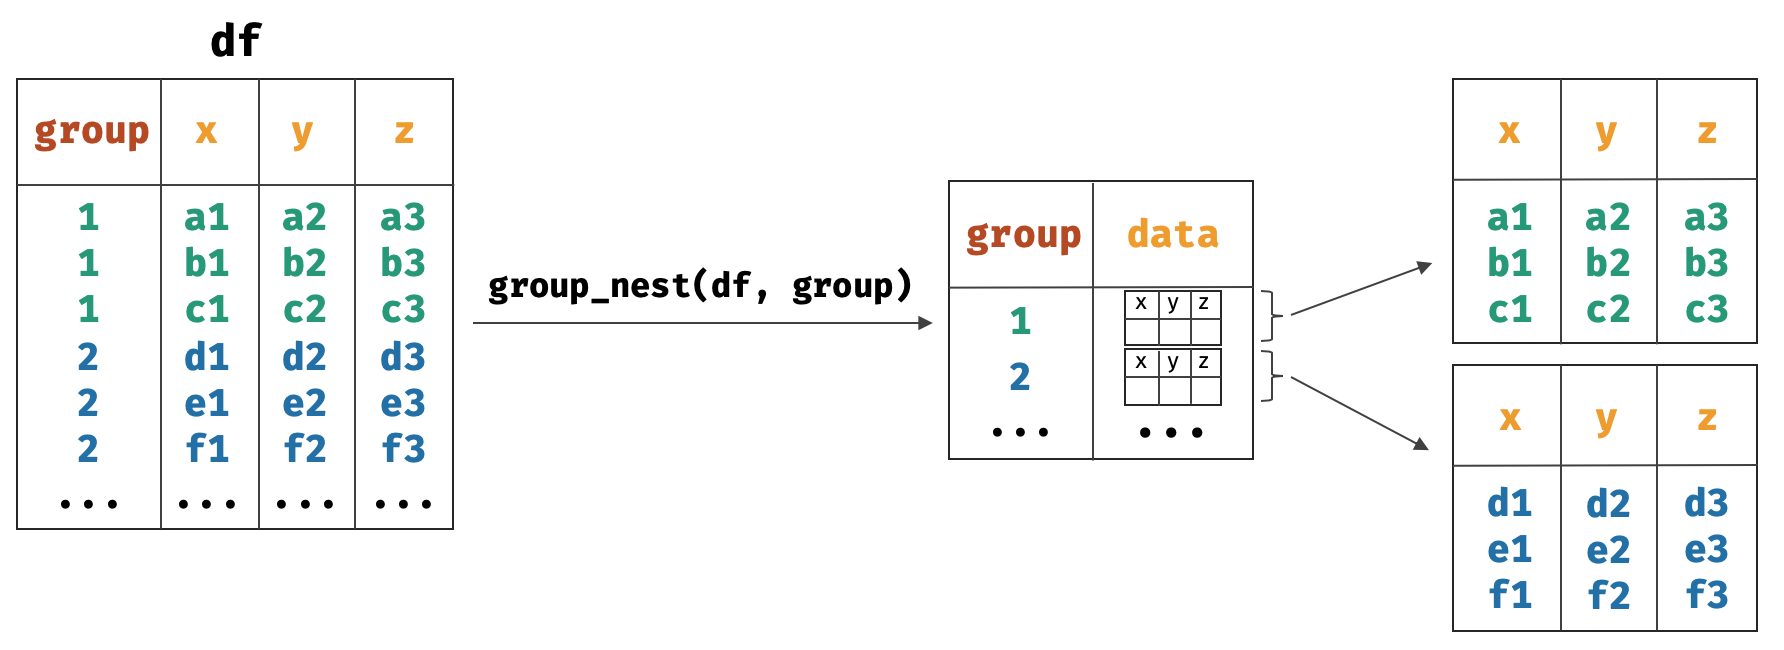
\includegraphics[width=\textwidth]{fig_process.png}
  \caption{Diagram of one approach to creating a list-column in a data frame (i.e. creating a nested data frame).}
  \label{process}
\end{figure}

Overall, this function is efficient and fast but by using \texttt{data.table} it can be somewhat faster. This will be shown using the following function:

\begin{Shaded}
\begin{Highlighting}[]
\NormalTok{group_nest_dt <-}\StringTok{ }\ControlFlowTok{function}\NormalTok{(dt, ..., }\DataTypeTok{.key =} \StringTok{"data"}\NormalTok{)\{}
  \KeywordTok{stopifnot}\NormalTok{(}\KeywordTok{is.data.table}\NormalTok{(dt))}

\NormalTok{  by <-}\StringTok{ }\KeywordTok{substitute}\NormalTok{(}\KeywordTok{list}\NormalTok{(...))}
  
\NormalTok{  express <-}\StringTok{ }\NormalTok{dt[, }\KeywordTok{list}\NormalTok{(}\KeywordTok{list}\NormalTok{(.SD)), by =}\StringTok{ }\KeywordTok{eval}\NormalTok{(by)]}
  \KeywordTok{setnames}\NormalTok{(express, }\DataTypeTok{old =} \StringTok{"V1"}\NormalTok{, }\DataTypeTok{new =}\NormalTok{ .key)}
\NormalTok{  express}
\NormalTok{\}}
\end{Highlighting}
\end{Shaded}

In essence, this function takes a data table, then creates a list of the data table per group specified in the \texttt{by} argument.

\begin{Shaded}
\begin{Highlighting}[]
\KeywordTok{group_nest_dt}\NormalTok{(players, team) }\OperatorTok\StringTok{ }
\StringTok{  }\KeywordTok{head}\NormalTok{()}
\end{Highlighting}
\end{Shaded}

\begin{verbatim}
##    team         data
## 1:  Min <data.table>
## 2:  Orl <data.table>
## 3:  Dal <data.table>
## 4:  Hou <data.table>
## 5:  Bos <data.table>
## 6:  Ind <data.table>
\end{verbatim}

This is nearly identical to the \texttt{dplyr::group\_nest()} function, in terms of output, but has data tables in the list-column instead of tibbles.

\begin{Shaded}
\begin{Highlighting}[]
\KeywordTok{group_nest}\NormalTok{(players, team) }\OperatorTok\StringTok{ }
\StringTok{  }\KeywordTok{head}\NormalTok{()}
\end{Highlighting}
\end{Shaded}

\begin{verbatim}
## # A tibble: 6 x 2
##   team  data              
##   <chr> <list>            
## 1 Atl   <tibble [44 x 30]>
## 2 Bos   <tibble [37 x 30]>
## 3 Bro   <tibble [41 x 30]>
## 4 Cha   <tibble [34 x 30]>
## 5 Chi   <tibble [43 x 30]>
## 6 Cle   <tibble [49 x 30]>
\end{verbatim}

Importantly, Figure \ref{speed} presents the timings from \texttt{bench::mark()} across the two approaches, showing \texttt{group\_nest\_dt()} is often faster. The memory allocated is very similar, with \texttt{group\_nest\_dt()} allocating 451KB and \texttt{group\_nest()} allocating 335KB.

\begin{figure}[tb]
  \centering
  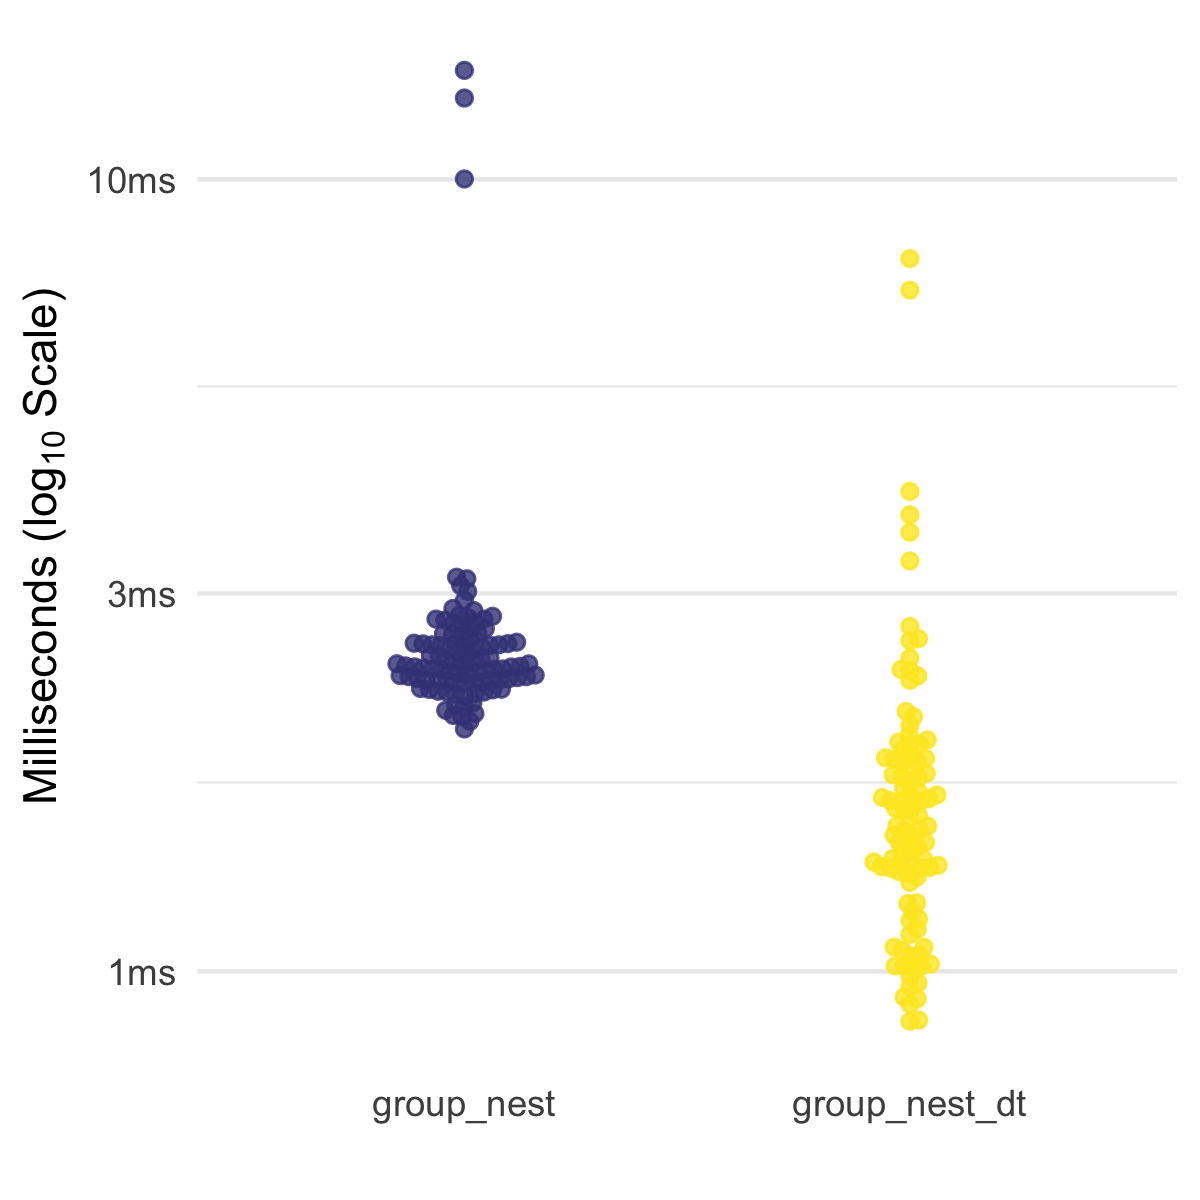
\includegraphics[width=0.6\textwidth]{timings_manuscript.png}
  \caption{Speed comparisons for each nesting approach. Note the scale of the y-axis is log$_{10}$.}
  \label{speed}
\end{figure}

This nesting approach can be used with multiple grouping variables too. For example, I show how a user could nest by both \texttt{team} and \texttt{year}, as is done below.

\begin{Shaded}
\begin{Highlighting}[]
\KeywordTok{group_nest_dt}\NormalTok{(players, team, year) }\OperatorTok\StringTok{ }
\StringTok{  }\KeywordTok{head}\NormalTok{()}
\end{Highlighting}
\end{Shaded}

\begin{verbatim}
##    team year         data
## 1:  Min 2018 <data.table>
## 2:  Orl 2018 <data.table>
## 3:  Dal 2018 <data.table>
## 4:  Hou 2018 <data.table>
## 5:  Bos 2018 <data.table>
## 6:  Ind 2018 <data.table>
\end{verbatim}

\hypertarget{modeling-within-the-nest}{%
\subsection{Modeling within the Nest}\label{modeling-within-the-nest}}

Often, the nested data can provide an intuitive format to run several models to understand key features of the data within the groups. Below, the relationship between points-per-game and assists-per-game for each team and year is modeled and then the \(R^2\) of the models are extracted. Since \texttt{performance::r2()} provides two versions of \(R^2\), I then grab only the first of the two.

\begin{Shaded}
\begin{Highlighting}[]
\NormalTok{players_nested <-}\StringTok{ }\KeywordTok{group_nest_dt}\NormalTok{(players, team, year) }\OperatorTok\StringTok{ }
\StringTok{  }\NormalTok{.[, ppg_apg    }\OperatorTok{:}\ErrorTok{=}\StringTok{ }\NormalTok{purrr}\OperatorTok{::}\KeywordTok{map}\NormalTok{(data, }\OperatorTok{~}\KeywordTok{lm}\NormalTok{(ppg }\OperatorTok{~}\StringTok{ }\NormalTok{apg, }\DataTypeTok{data =}\NormalTok{ .x))] }\OperatorTok\StringTok{ }
\StringTok{  }\NormalTok{.[, r2_list    }\OperatorTok{:}\ErrorTok{=}\StringTok{ }\NormalTok{purrr}\OperatorTok{::}\KeywordTok{map}\NormalTok{(ppg_apg, }\OperatorTok{~}\NormalTok{performance}\OperatorTok{::}\KeywordTok{r2}\NormalTok{(.x))] }\OperatorTok\StringTok{ }
\StringTok{  }\NormalTok{.[, r2_ppg_apg }\OperatorTok{:}\ErrorTok{=}\StringTok{ }\NormalTok{purrr}\OperatorTok{::}\KeywordTok{map_dbl}\NormalTok{(r2_list, }\OperatorTok{~}\NormalTok{.x[[}\DecValTok{1}\NormalTok{]])]}
\KeywordTok{head}\NormalTok{(players_nested)}
\end{Highlighting}
\end{Shaded}

\begin{verbatim}
##    team year         data ppg_apg      r2_list r2_ppg_apg
## 1:  Min 2018 <data.table>    <lm> <r2_generic>  0.4662060
## 2:  Orl 2018 <data.table>    <lm> <r2_generic>  0.4357684
## 3:  Dal 2018 <data.table>    <lm> <r2_generic>  0.4305347
## 4:  Hou 2018 <data.table>    <lm> <r2_generic>  0.6967150
## 5:  Bos 2018 <data.table>    <lm> <r2_generic>  0.6043402
## 6:  Ind 2018 <data.table>    <lm> <r2_generic>  0.6060465
\end{verbatim}

\noindent This produces two list-columns (\texttt{ppg\_apg} and \texttt{r2\_list}) and a numeric vector (\texttt{r2\_ppg\_apg}) all organized by team and year. This information is then readily available to plot. For example, one can look at how related points-per-game and assists-per-game are by team and year--in essence, showing which teams have players who both score and assist. This example is shown in Figure \ref{exfig}.

\begin{figure}[tb]
  \centering
  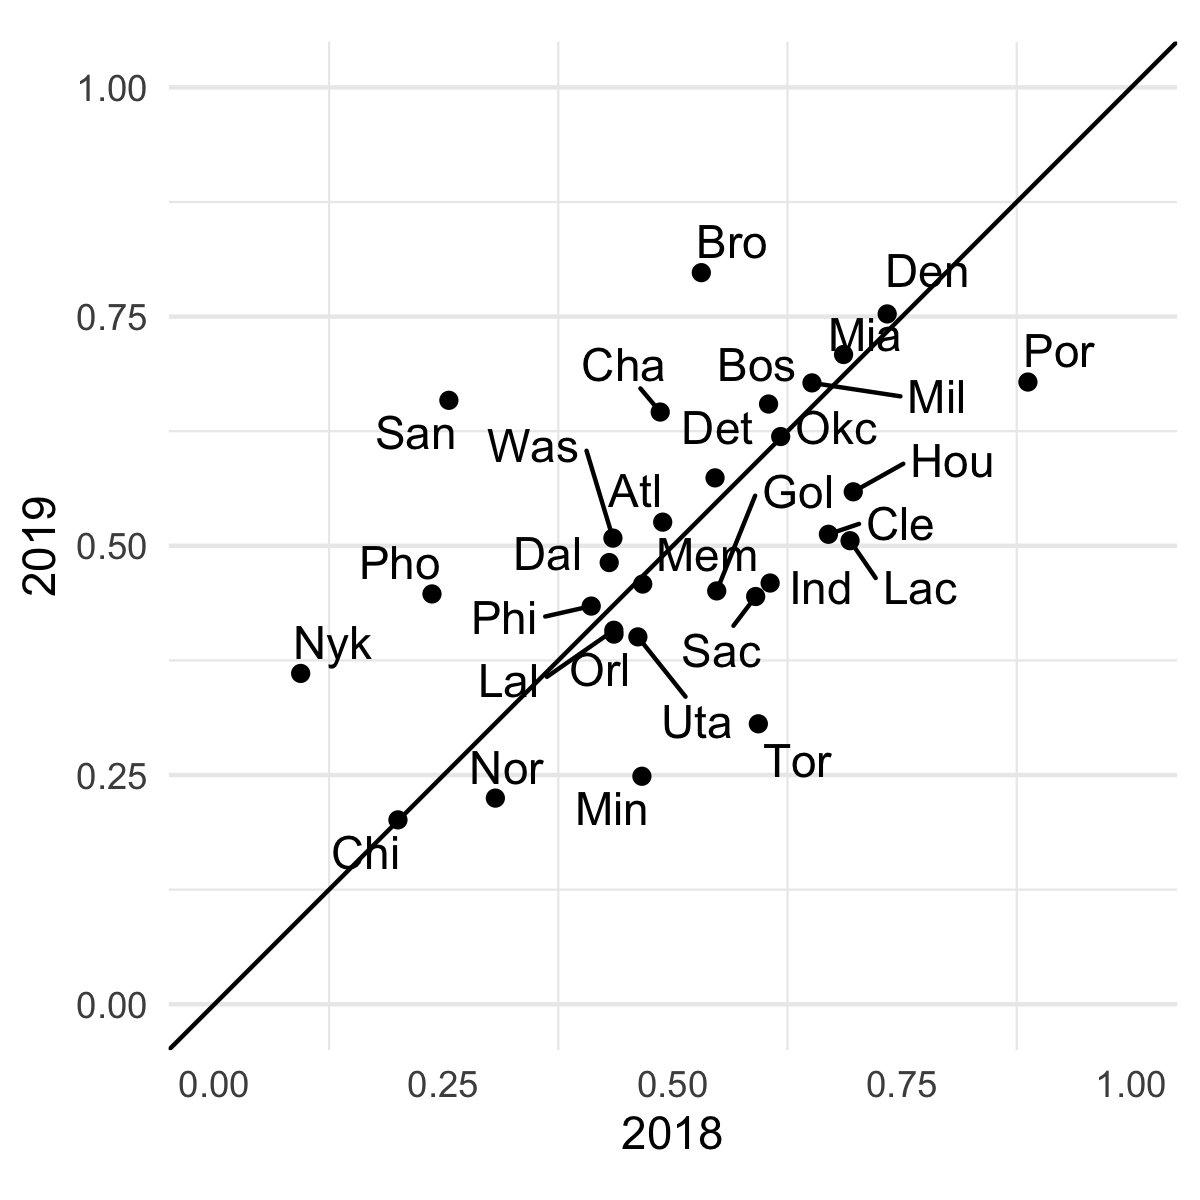
\includegraphics[width=0.5\textwidth]{ex_fig.png}
  \caption{Example analysis performed using nested data to provide information for each team and year.}
  \label{exfig}
\end{figure}

\hypertarget{unnest-with-data.table}{%
\section{\texorpdfstring{Unnest with \texttt{data.table}}{Unnest with data.table}}\label{unnest-with-data.table}}

After performing the manipulations or analyses within the nest, it can often be good to unnest to finalize analyses. Again, like with \texttt{group\_nest\_dt()}, this \texttt{unnest\_dt()} function relies solely on the syntax of \texttt{data.table}, using the \texttt{j} and \texttt{by} arguments as shown below.

\begin{Shaded}
\begin{Highlighting}[]
\NormalTok{unnest_dt <-}\StringTok{ }\ControlFlowTok{function}\NormalTok{(dt, col, id)\{}
  \KeywordTok{stopifnot}\NormalTok{(}\KeywordTok{is.data.table}\NormalTok{(dt))}
  
\NormalTok{  by <-}\StringTok{ }\KeywordTok{substitute}\NormalTok{(id)}
\NormalTok{  col <-}\StringTok{ }\KeywordTok{substitute}\NormalTok{(}\KeywordTok{unlist}\NormalTok{(col, }\DataTypeTok{recursive =} \OtherTok{FALSE}\NormalTok{))}
  
\NormalTok{  dt[, }\KeywordTok{eval}\NormalTok{(col), by =}\StringTok{ }\KeywordTok{eval}\NormalTok{(by)]}
\NormalTok{\}}
\end{Highlighting}
\end{Shaded}

This function can be used to unnest a data table, like the \texttt{players\_nested} data table from earlier where the nested column is a data table, data frame, or tibble. Below, the \texttt{data} column in the table is unnested by \texttt{team} and \texttt{year} and then I select just a few of the variables.

\begin{Shaded}
\begin{Highlighting}[]
\KeywordTok{unnest_dt}\NormalTok{(players_nested, }
          \DataTypeTok{col =}\NormalTok{ data, }
          \DataTypeTok{id =} \KeywordTok{list}\NormalTok{(team, year)) }\OperatorTok\StringTok{ }
\StringTok{  }\NormalTok{.[, .(team, year, full_name, pos, age, gp, mpg)]}
\end{Highlighting}
\end{Shaded}

\begin{verbatim}
##       team year          full_name pos   age gp  mpg
##    1:  Min 2018       Aaron Brooks  PG 33.00 32  5.9
##    2:  Min 2018     Andrew Wiggins  SF 22.00 82 36.3
##    3:  Min 2018      Anthony Brown  SF 25.00  1  3.7
##    4:  Min 2018       Cole Aldrich   C 29.00 21  2.3
##    5:  Min 2018       Derrick Rose  PG 29.00  9 12.4
##   ---                                               
## 1223:  Det 2019     Svi Mykhailiuk   G 21.84  3  6.6
## 1224:  Det 2019      Zaza Pachulia   C 35.16 68 12.9
## 1225:  Det 2019 Glenn Robinson III G-F 25.26 47 13.0
## 1226:  Det 2019          Ish Smith   G 30.77 56 22.3
## 1227:  Det 2019       Khyri Thomas   G 22.92 26  7.5
\end{verbatim}

\begin{figure}[tb]
  \centering
  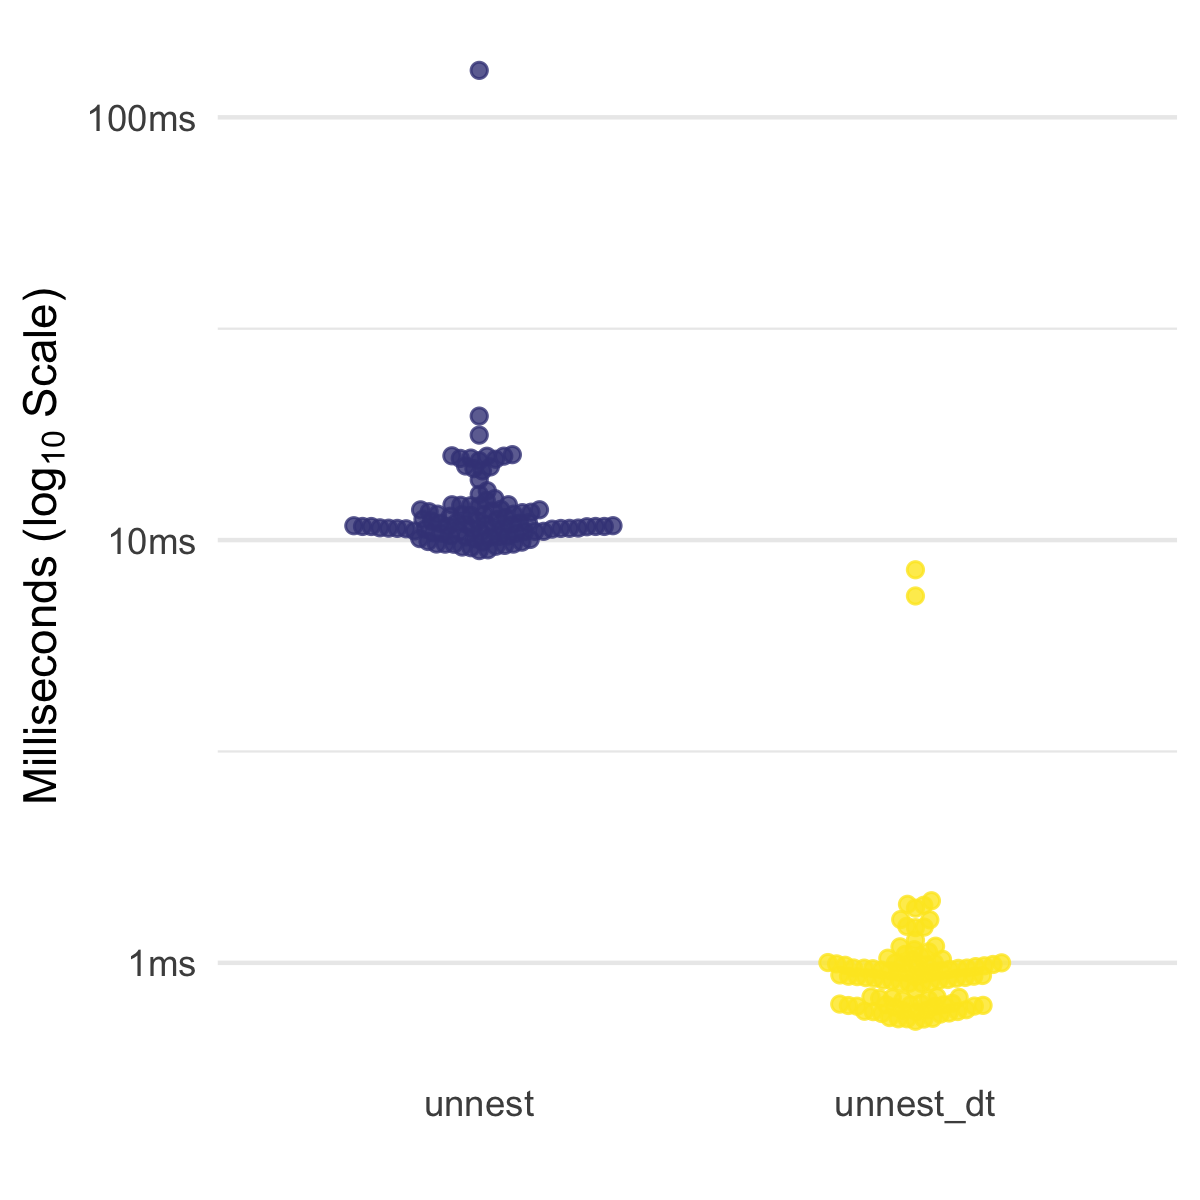
\includegraphics[width=0.6\textwidth]{timings_unnest_manuscript.png}
  \caption{Speed comparisons for each unnesting approach. Note the scale of the y-axis is log$_{10}$.}
  \label{speed2}
\end{figure}

Again, this function is quick and efficient. Figure \ref{speed2} presents the timings from \texttt{bench::mark()} across the two unnesting approaches, showing the \texttt{data.table} approach is often faster. The memory allocated is about half for the \texttt{data.table} approach here, with \texttt{unnest\_dt()} allocating 912KB and \texttt{tidyr::unnest()} allocating 1.83MB.

A slight variation of this function can be used for list-columns with atomic vectors instead of data tables. A function like the following works well.

\begin{Shaded}
\begin{Highlighting}[]
\NormalTok{unnest_vec_dt <-}\StringTok{ }\ControlFlowTok{function}\NormalTok{(dt, cols, id, nam)\{}
  \KeywordTok{stopifnot}\NormalTok{(}\KeywordTok{is.data.table}\NormalTok{(dt))}
  
\NormalTok{  by <-}\StringTok{ }\KeywordTok{substitute}\NormalTok{(id)}
\NormalTok{  cols <-}\StringTok{ }\KeywordTok{substitute}\NormalTok{(}\KeywordTok{unlist}\NormalTok{(cols, }\DataTypeTok{recursive =} \OtherTok{FALSE}\NormalTok{, }\DataTypeTok{use.names =} \OtherTok{FALSE}\NormalTok{))}
  
\NormalTok{  express <-}\StringTok{ }\NormalTok{dt[, }\KeywordTok{eval}\NormalTok{(cols), by =}\StringTok{ }\KeywordTok{eval}\NormalTok{(by)]}
  \KeywordTok{setnames}\NormalTok{(express, }\DataTypeTok{old =} \KeywordTok{paste0}\NormalTok{(}\StringTok{"V"}\NormalTok{, }\DecValTok{1}\OperatorTok{:}\KeywordTok{length}\NormalTok{(nam)), }\DataTypeTok{new =}\NormalTok{ nam)}
\NormalTok{  express}
\NormalTok{\}}
\end{Highlighting}
\end{Shaded}

In \texttt{players\_nested}, the \texttt{r2\_list} column is a list of numeric vectors. This can be unnested as shown below, providing the two measures of \(R^2\) per team per year.

\begin{Shaded}
\begin{Highlighting}[]
\KeywordTok{unnest_vec_dt}\NormalTok{(players_nested, }
              \DataTypeTok{cols =} \KeywordTok{list}\NormalTok{(r2_list), }
              \DataTypeTok{id =} \KeywordTok{list}\NormalTok{(team, year), }
              \DataTypeTok{nam =} \StringTok{"r2"}\NormalTok{)}
\end{Highlighting}
\end{Shaded}

\begin{verbatim}
##      team year        r2
##   1:  Min 2018  0.466206
##   2:  Min 2018 0.4280779
##   3:  Orl 2018 0.4357684
##   4:  Orl 2018 0.4025783
##   5:  Dal 2018 0.4305347
##  ---                    
## 116:  Lac 2019 0.4808586
## 117:  Phi 2019 0.4342685
## 118:  Phi 2019 0.4106964
## 119:  Det 2019 0.5740963
## 120:  Det 2019  0.550435
\end{verbatim}

\hypertarget{memory-usage-of-list-columns}{%
\section{Memory Usage of List-Columns}\label{memory-usage-of-list-columns}}

Last item to assess herein is the computer memory usage of different formats of data tables with the same data. We can use the following large data sets in wide format, nested wide format, long format, and nested wide format to make brief comparisons.

\begin{Shaded}
\begin{Highlighting}[]
\CommentTok{# Wide}
\NormalTok{wide_format <-}\StringTok{ }\KeywordTok{data.table}\NormalTok{(}\DataTypeTok{id =} \DecValTok{1}\OperatorTok{:}\FloatTok{1e6}\NormalTok{,}
                          \DataTypeTok{x1 =} \KeywordTok{rnorm}\NormalTok{(}\FloatTok{1e6}\NormalTok{),}
                          \DataTypeTok{x2 =} \KeywordTok{rnorm}\NormalTok{(}\FloatTok{1e6}\NormalTok{),}
                          \DataTypeTok{y1 =} \KeywordTok{rnorm}\NormalTok{(}\FloatTok{1e6}\NormalTok{),}
                          \DataTypeTok{y2 =} \KeywordTok{rnorm}\NormalTok{(}\FloatTok{1e6}\NormalTok{),}
                          \DataTypeTok{group =} \KeywordTok{rbinom}\NormalTok{(}\FloatTok{1e6}\NormalTok{, }\DecValTok{1}\NormalTok{, }\FloatTok{.5}\NormalTok{))}
\NormalTok{nested_wide_format <-}\StringTok{ }\KeywordTok{group_nest_dt}\NormalTok{(wide_format, group)}

\CommentTok{# Long}
\NormalTok{long_format <-}\StringTok{ }\KeywordTok{melt.data.table}\NormalTok{(wide_format, }
                               \DataTypeTok{id.vars =} \KeywordTok{c}\NormalTok{(}\StringTok{"id"}\NormalTok{, }\StringTok{"group"}\NormalTok{),}
                               \DataTypeTok{measure.vars =} \KeywordTok{c}\NormalTok{(}\StringTok{"x1"}\NormalTok{, }\StringTok{"x2"}\NormalTok{, }\StringTok{"y1"}\NormalTok{, }\StringTok{"y2"}\NormalTok{))}
\NormalTok{nested_long_format <-}\StringTok{ }\KeywordTok{group_nest_dt}\NormalTok{(long_format, group)}
\end{Highlighting}
\end{Shaded}

I use the \texttt{lobstr} package to assess the object size of each format of the same data, shown in the output below.

\begin{verbatim}
##                Format Memory (MB)
## 1:        wide_format      40.002
## 2: nested_wide_format      36.003
## 3:        long_format      80.001
## 4: nested_long_format      64.003
\end{verbatim}

Not surprising, the memory usage of nested data is lower than for its none nested corresponding data. This is directly related to the reduction in redundancies in the data otherwise there. That is, the nested data has far fewer rows containing the \texttt{group} variable. That, alone, in this large data saves memory. For example, the size of a single column of the \texttt{group} variable in wide format is 4 MB; and in long format it is 16 MB By reducing a single variable in this case, we save several megabytes of memory.

\hypertarget{discussion}{%
\section{Discussion}\label{discussion}}

List-columns are a useful approach to structuring data into a format that can be safely cleaned, manipulated, and analyzed by groups. It also provides for a more cognitively efficient way for a user to understand their data, allowing large data to be represented more concisely within groups.

The \texttt{tidyverse} provides several functions to work with nested data, which are relatively quick and efficient. For most data situations, these functions will do all that a user will need. However, in some situations, \texttt{data.table} can perform needed manipulations and analyses that cannot otherwise be done or that would take too long to complete. In these situations, and for users that prefer to use \texttt{data.table}, this tutorial can help provide direction in using list-columns.

Furthermore, as expected, the memory usage of nested data is lower than for its none nested corresponding data. This is due to the reduction in the redundancies present in wide and long format. This suggests that it is not only the cognitive benefits to the user that makes this format more efficient.

\hypertarget{limitations}{%
\subsection{Limitations}\label{limitations}}

There are some notable limitations to list-columns in general, and in \texttt{data.table} specifically. First, the three custom functions built on \texttt{data.table} presented herein are not well-tested and are certainly not expected to work in each case where \texttt{dplyr::group\_nest()}, \texttt{tidyr::unnest()}, and other tidy functions would work. Rather, they were presented to show how a user can leverage the speed and efficiency of \texttt{data.table} to create, and work with, list-columns.

Second, it is important to realize that nested data can remove the ability to use vectorization across groups. Depending on the analyses being conducted, this may slow down the computation to the point that nested data actually is a hindrance to performance.

Finally, when using list-columns in tibbles, the print method provides the dimensions of each corresponding nested tibble. This method is helpful in understanding the nested data without any need to extract it. This could be a minor, but valuable, update to the print method in \texttt{data.table}.

\hypertarget{conclusions}{%
\section{Conclusions}\label{conclusions}}

The use of list-columns in \texttt{data.table} is very similar to that in the \texttt{tidyverse}. It provides speed and efficiency in both nesting and unnesting the data, and can be used with the \texttt{purrr::map*()} and other powerful functions.

\hypertarget{references}{%
\section{References}\label{references}}

\begingroup
\setlength{\parindent}{-0.5in}
\setlength{\leftskip}{0.5in}

\hypertarget{refs}{}
\leavevmode\hypertarget{ref-R-papaja}{}%
Aust, F., \& Barth, M. (2018). \emph{papaja: Create APA manuscripts with R Markdown}. Retrieved from \url{https://github.com/crsh/papaja}

\leavevmode\hypertarget{ref-jenny}{}%
Bryan, J. (2018). List columns (as part of "purrr tutorial"). Retrieved from \url{https://jennybc.github.io/purrr-tutorial/ls13_list-columns.html}

\leavevmode\hypertarget{ref-R-ggbeeswarm}{}%
Clarke, E., \& Sherrill-Mix, S. (2017). \emph{Ggbeeswarm: Categorical scatter (violin point) plots}. Retrieved from \url{https://github.com/eclarke/ggbeeswarm}

\leavevmode\hypertarget{ref-R-data.table}{}%
Dowle, M., \& Srinivasan, A. (2019). \emph{Data.table: Extension of `data.frame`}. Retrieved from \url{https://CRAN.R-project.org/package=data.table}

\leavevmode\hypertarget{ref-R-bench}{}%
Hester, J. (2019). \emph{Bench: High precision timing of r expressions}. Retrieved from \url{https://CRAN.R-project.org/package=bench}

\leavevmode\hypertarget{ref-R-performance}{}%
Lüdecke, D., Makowski, D., \& Waggoner, P. (2019). \emph{Performance: Assessment of regression models performance}. Retrieved from \url{https://easystats.github.io/performance/}

\leavevmode\hypertarget{ref-R-base}{}%
R Core Team. (2018). \emph{R: A language and environment for statistical computing}. Vienna, Austria: R Foundation for Statistical Computing. Retrieved from \url{https://www.R-project.org/}

\leavevmode\hypertarget{ref-R-ggplot2}{}%
Wickham, H. (2016). \emph{Ggplot2: Elegant graphics for data analysis}. Springer-Verlag New York. Retrieved from \url{https://ggplot2.tidyverse.org}

\leavevmode\hypertarget{ref-R-lobstr}{}%
Wickham, H. (2019a). \emph{Lobstr: Visualize r data structures with trees}. Retrieved from \url{https://CRAN.R-project.org/package=lobstr}

\leavevmode\hypertarget{ref-R-rvest}{}%
Wickham, H. (2019b). \emph{Rvest: Easily harvest (scrape) web pages}. Retrieved from \url{https://CRAN.R-project.org/package=rvest}

\leavevmode\hypertarget{ref-R-stringr}{}%
Wickham, H. (2019c). \emph{Stringr: Simple, consistent wrappers for common string operations}. Retrieved from \url{https://CRAN.R-project.org/package=stringr}

\leavevmode\hypertarget{ref-R-dplyr}{}%
Wickham, H., François, R., Henry, L., \& Müller, K. (2019). \emph{Dplyr: A grammar of data manipulation}. Retrieved from \url{https://CRAN.R-project.org/package=dplyr}

\leavevmode\hypertarget{ref-R-tidyr}{}%
Wickham, H., \& Henry, L. (2019). \emph{Tidyr: Tidy messy data}. Retrieved from \url{https://CRAN.R-project.org/package=tidyr}

\endgroup


\end{document}
